\section{Introdução à Lógica de Primeira Ordem} % Necessário para gerar o \tableofcontents

\begin{frame}[t]
\vskip 3cm
\begin{center}
{\Huge Introdução à\\Lógica de Primeira Ordem}
\end{center}
\end{frame}

\subsection{Sentenças Abertas}

\begin{frame}[t]{Lógica de Primeira Ordem}
	\begin{itemize} \itemsep 0.4cm
	\item Lógica de Primeira Ordem (LPO) é uma extensão à Lógica Proposicional onde cada proposição $p, q, r, \ldots$ é entendida como um conjunto de proposições pertencentes a um dado conjunto (chamado de {\bf domínio}) $$p(x):~ x \in A$$

	\item $p(x)$ é uma {\bf sentença aberta} em um conjunto $A$, se e somente se, $p(x)$ se torna uma proposição \underline{para todo} $x=a, a \in A$

	\item Se $a \in A$ e $\Phi(p(a)) = \mbox{verdade}$ diz-se que $a$ {\bf satisfaz} $p(x)$

	\item Exemplo: seja $N = 1, 2, 3, \ldots$
	\begin{itemize}
	\item $x + 1 > 8$
	\item $x^2 - 5x + 6 = 0$
	\end{itemize}
	\end{itemize}
\end{frame}

\begin{frame}[t]{Conjunto-Verdade para Sentenças Abertas}
	\begin{itemize} \itemsep 0.7cm
	\item É definido com o conjunto $(V_p)$ de todos os elementos $a \in A$ tais que $\Phi(p(a)) = \mbox{verdade}$

	\item Exemplo: $x + 1 > 8$ em $N$ (números naturais)
	\begin{itemize}
	\item $V_p = \{ x \mid x \in N \wedge x + 1 > 8\} = \{8, 9, 10, \ldots\}$
	\end{itemize}

	\item Considerações
	\begin{description}
	\item [Condição Universal] $V_p = A$, $\Phi(p(x))$ é verdade para {\bf todo} $x \in A$
	\item [Condição Possível]  $V_p \subset A$, $\Phi(p(x))$ é verdade para {\bf algum} $x \in A$
	\item [Condição Impossível] $V_p = \phi$, $\Phi(p(x))$ é verdade para {\bf nenhum} $x \in A$
	\end{description}
	\end{itemize}
\end{frame}

\begin{frame}[t]{Sentenças Abertas -- Duas Variáveis}
	\begin{itemize} \itemsep 0.4cm
	\item $p(x,y)$ é uma sentença aberta em dois domínios $A$ e $B$, se e somente se, $p(x,y)$ se torna uma proposição para todo par $(a,b) \in A \times B$

	\item Se $a \in A, b \in B ~e~ \Phi(p(a,b)) = \mbox{verdade}$ diz-se que $(a,b)$ satisfaz $p(x,y)$

	\item Exemplo: seja $A = \{1, 2, 3\}$ e $B = \{5, 6\}$
	\begin{itemize}
	\item $x < y$
	\item $y = 2x$
	\end{itemize}
	\end{itemize}
\end{frame}

\begin{frame}[t]{Conjunto-Verdade para Sentenças Abertas}
	\begin{itemize} \itemsep 0.7cm
	\item É o conjunto $(V_p)$ de todos os elementos $(a, b) \in A \times B$ tais que $\Phi(p(a,b)) = \mbox{verdade}$ $$V_p = \{(x,y) \mid x \in A \wedge y \in B \wedge \Phi(p(x,y)) \}$$

	\item Considerações
	\begin{description}
	\item [Condição Universal] $V_p = A \times B$, $\Phi(p(x,y))$ é verdade para {\bf todo} $(x,y) \in A \times B$
	\item [Condição Possível]  $V_p \subset A \times B$, $\Phi(p(x,y))$ é verdade para {\bf algum} $(x,y) \in A \times B$
	\item [Condição Impossível] $V_p = \phi$, $\Phi(p(x,y))$ é verdade para {\bf nenhum} $(x,y) \in A \times B$
	\end{description}
	\end{itemize}
\end{frame}

\begin{frame}[t]{Sentenças Abertas -- N-Variáveis}
	\begin{itemize} \itemsep 0.4cm
	\item $p(x_1, x_2, \ldots, x_N)$ é uma sentença aberta em $N$ domínios $A_1, A_2, \ldots, A_N$, se e somente se, $p(x_1, x_2, \ldots, x_N)$ se torna uma proposição para toda tupla $(a_1, a_2, \ldots, a_N) \in A_1 \times A_2 \times \ldots \times A_N$
	\end{itemize}
\end{frame}

\begin{frame}[t]{Exercícios}
	\begin{itemize}
	\item Determinar o conjunto-verdade ($V_p$) para
	\begin{enumerate}
	\item $2x = 6$
	\item $x - 1 < 4$
	\item $x^2 < 25$
	\end{enumerate}

	\item ...considerando:
	\begin{itemize}
	\item A = números naturais
	\item $A = \{ 1, 3, 4, 7, 9, 11 \}$
	\end{itemize}
	\end{itemize}
\end{frame}

\begin{frame}[t]{Operações Lógicas sobre Sentenças Abertas}
	\begin{itemize}
	\item {\bf Conjunção} $$V_{p \wedge q} = V_p \cap V_q = \{ x \in A \mid p(x) \} \cap \{ x \in A \mid q(x) \}$$

	\item {\bf Disjunção}  $$V_{p \vee q} = V_p \cup V_q = \{ x \in A \mid p(x) \} \cup \{ x \in A \mid q(x) \}$$

	\item {\bf Negação} $$V_{\sim p} = \bar{A} = \{ x \in A \mid A - p(x) \}$$
	\end{itemize}
\end{frame}

\begin{frame}[t]{Operações Lógicas sobre Sentenças Abertas}
	\begin{itemize}
	\item {\bf Condicional} 
	\begin{itemize}
	\item Se $p(x) \rightarrow q(x)$ então $\sim p(x) \vee q(x)$
	$$V_{p \rightarrow q} = V_{\sim p} \cup V_q = \{ x \in A \mid A - p(x) \} \cup \{ x \in A \mid q(x) \}$$
	\end{itemize}

	\item {\bf Bicondicional} 
	\begin{itemize}
	\item Se $p(x) \leftrightarrow q(x)$ então $(p(x) \rightarrow q(x)) \wedge (q(x) \rightarrow p(x))$
	$$V_{p \leftrightarrow q} = (V_{\sim p} \cup V_q) \cap (V_{\sim q} \cup V_p)$$
	\end{itemize}
	\end{itemize}

	\hskip 1.5cm

	\begin{center}
	{\bf A álgebra das proposições que era válida para proposições atômicas e compostas, continua válida para sentenças abertas}
	\end{center}
\end{frame}

\begin{frame}[t]{Exercícios}
	\begin{itemize}
	\item Determina o conjunto-verdade para $A = \{1 \ldots 10 \}$
	\begin{enumerate}
	\item $x < 7 \wedge \mbox{x é ímpar}$
	\item $\mbox{x é par} \wedge x + 2 \leq 10$
	\item $\mbox{x é primo} \vee x + 5 \in A$
	\item $\sim (\mbox{x é primo})$
	\item $\sim (x^2 - 3x = 0)$
	\item $x + 5 \in A \rightarrow x < 0$
	\item $x^2 < 12 \leftrightarrow x^2 - 5x + 6 = 0$
	\end{enumerate}
	\end{itemize}
\end{frame}

\begin{frame}[t]{Quantificadores}
	\begin{itemize} \itemsep 0.8cm
	\item Expressam relações lógicas de \underline{quantidade} entre variáveis e seus respectivos domínios
	\item Tipos:
	\begin{itemize}
	\item Quantificador Universal ($\forall$)
	\item Quantificador Existencial ($\exists$)
	\end{itemize}
	\end{itemize}
\end{frame}

\begin{frame}[t]{Quantificador Universal}
	\begin{itemize} \itemsep 0.8cm
	\item Para uma sentença aberta $p(x)$ em um conjunto não-vazio $A$, onde para {\bf todo} elemento $x \in A$, temos $\Phi(p(x)) = \mbox{verdade}$
	\begin{itemize}
	\item $\Phi(\forall x \in A: p(x)) \equiv p(x_1) \wedge p(x_2) \wedge p(x_3) \wedge \ldots \wedge p(x_N)$
	\item ou simplesmente $\Phi(\forall x: p(x))$
	\item conclui-se que $V_p = A$
	\end{itemize}

	\item Exemplo: ``{\it Todo x é mortal no domínio dos seres humanos}''
	\end{itemize}
\end{frame}

\begin{frame}[t]{Quantificador Universal - Exercício}
	\begin{itemize}
	\item Seja D = [ 10 \ldots 15 ] $$\forall x \in D: \frac{x}{2} \geq 5$$ Interprete e avalia a validade da expressão acima
	\end{itemize}
\end{frame}

\begin{frame}[t]{Quantificador Universal - Exercício}
	\begin{itemize} \itemsep 0.7cm
	\item Seja D = [ 10 \ldots 15 ] $$\forall x \in D: \frac{x}{2} \geq 5$$ Interprete e avalia a validade da expressão acima

	\item {\scriptsize $\Phi(\forall x \in D: \frac{x}{2} \geq 5) = \Phi(\frac{10}{2} \geq 5) \wedge \Phi(\frac{11}{2} \geq 5) \wedge \Phi(\frac{12}{2} \geq 5) \wedge \Phi(\frac{13}{2} \geq 5) \wedge \Phi(\frac{14}{2} \geq 5) \wedge \Phi(\frac{15}{2} \geq 5)$}
	\end{itemize}
\end{frame}

\begin{frame}[t]{Quantificador Universal - Exercício}
	\begin{itemize} \itemsep 0.7cm
	\item Seja D = [ 10 \ldots 15 ] $$\forall x \in D: \frac{x}{2} \geq 5$$ Interprete e avalia a validade da expressão acima

	\item {\scriptsize $\Phi(\forall x \in D: \frac{x}{2} \geq 5) = \Phi(\frac{10}{2} \geq 5) \wedge \Phi(\frac{11}{2} \geq 5) \wedge \Phi(\frac{12}{2} \geq 5) \wedge \Phi(\frac{13}{2} \geq 5) \wedge \Phi(\frac{14}{2} \geq 5) \wedge \Phi(\frac{15}{2} \geq 5)$}

	\item $\Phi(\forall x \in D: \frac{x}{2} \geq 5) = V \wedge V \wedge V \wedge V \wedge V \wedge V  = V$
	\end{itemize}
\end{frame}

\begin{frame}[t]{Quantificador Existencial}
	\begin{itemize} \itemsep 0.8cm
	\item Para uma sentença aberta $p(x)$ em um conjunto não-vazio $A$, onde para {\bf pelo menos um} elemento $x \in A$, temos $\Phi(p(x)) = \mbox{verdade}$
	\begin{itemize}
	\item $\Phi(\exists x \in A: p(x)) \equiv p(x_1) \vee p(x_2) \vee p(x_3) \vee \ldots \vee p(x_N)$
	\item ou simplesmente $\Phi(\exists x: p(x))$
	\item conclui-se que $V_p \subset A$
	\end{itemize}

	\item Exemplo: ``{\it Existe pelo menos um x que é homem no domínio dos seres humanos}''
	\end{itemize}
\end{frame}

\begin{frame}[t]{Quantificador Existencial - Exercício}
	\begin{itemize}
	\item Seja D = [ 10 \ldots 15 ] $$\exists x \in D: mod(x,3) = 0$$ Interprete e avalia a validade da expressão acima
	\end{itemize}
\end{frame}

\begin{frame}[t]{Quantificador Existencial - Exercício}
	\begin{itemize}\itemsep 0.7cm
	\item Seja D = [ 10 \ldots 15 ] $$\exists x \in D: mod(x,3) = 0$$ Interprete e avalia a validade da expressão acima

	\item {\scriptsize $\Phi(\exists x \in D: mod(x,3) = 0) = \Phi(mod(10,3) = 0) \vee \Phi(mod(11,3) = 0) \vee \Phi(mod(12,3) = 0) \vee \Phi(mod(13,3) = 0) \vee \Phi(mod(14,3) = 0) \vee \Phi(mod(15,3) = 0)$}

	\item $\Phi(\exists x \in D: mod(x,3) = 0) = F \vee F \vee V \vee F \vee F \vee V  =  V$
	\end{itemize}
\end{frame}

\begin{frame}[t]{Variável Ligada e Variável Livre}
	\begin{itemize}
	\item Se há um quantificador incidindo sobre uma variável, essa se chama {\bf variável ligada}. Caso contrário, chama-se {\bf variável livre}

	\item Em outras palavras, variáveis ligadas estarão \underline{sempre} associadas a domínios, e portanto para tais é possível a sua interpretação ($\Phi$)

	\item Exemplos: $$\exists x \in A: 3x + 1 > 10$$ $$x + 3 = -4$$

	\item Princípio da Substituição de Variáveis Ligadas
	\begin{itemize}
	\item $\forall x \in A: p(x) \Leftrightarrow \forall y \in A: p(y)$
	\item $\exists x \in A: p(x) \Leftrightarrow \exists y \in A: p(y)$
	\end{itemize}
	\end{itemize}
\end{frame}

\begin{frame}[t]{Quantificador de Existência e Unicidade}
	\begin{itemize}\itemsep 1cm
	\item Para $x^2 = 16$ sobre o conjunto dos números reais ($\Re$) temos: $$4^2 = 16 \wedge (-4)^2 = 16 \Leftrightarrow 4 \neq -4$$ portanto conclui-se que: $$\exists x,y \in \Re: (x^2 = 16 \wedge y^2 = 16 \wedge x \neq y)$$

	\item Para $x^3 = 27$ temos: $$\exists x \in\Re: (x^3 = 27)$$ $$(x^3 = 27) \wedge (y^3 = 27) \rightarrow (x = y)$$ portanto: $$\exists ! x \in\Re: (x^3 = 27)$$
	\end{itemize}
\end{frame}

\begin{frame}[t]{Negação de Quantificadores}
	\begin{itemize}
	\item Regra de DE MORGAN para quantificadores
	\item $\sim (\forall x \in A: p(x)) \Leftrightarrow \exists x \in A: \sim p(x)$
	\item $\sim (\exists x \in A: p(x)) \Leftrightarrow \forall x \in A: \sim p(x)$
	\end{itemize}
\end{frame}

\begin{frame}[t]{Quantificadores -- N-Variáveis}
	\begin{description} \itemsep 1.3cm
	\item [Quantificação Parcial]  $$\exists x \in A: (2x + y < 7),$$ $$\mbox{ onde } A = \{ 1 \ldots 5 \}$$

	\item [Quantificação Múltipla] $$\exists x \in A, \forall y \in B: (2x + y < 7),$$ $$\mbox{ onde } A = \{ 1 \ldots 5 \}, B = \{ 3, 4, 5 \}$$
	\end{description}
\end{frame}

\begin{frame}[t]{Negação de Múltiplos Quantificadores}
	\begin{itemize} \itemsep 0.8cm
	\item $\sim (\forall x \exists y: p(x,y)) \Leftrightarrow$

	\item $\exists x \sim (\exists y: p(x,y)) \Leftrightarrow$

	\item $\exists x \forall y: \sim p(x,y)$
	\end{itemize}
\end{frame}


\begin{frame}[t]{Simplificando a Notação da LPO}

Em alguns livros, a notação dos parênteses pode ser omitida, mas tome
muito cuidado. Veja os exemplos de simplificações:

	\begin{itemize} \itemsep 0.8cm
	\item $\forall x\:\: p(x) \equiv \forall x\:\: px $

	\item $\exists x \forall y \:\: p(x,y) \equiv \exists x \forall y \:\: pxy$

	\item $\exists x \forall y \exists z  \:\:   p(x,y,z) \equiv \exists x \forall y \exists z  \:\:  pxyz$
	
	\end{itemize}
	
	
	Em geral, vamos continuar usando os parênteses e vírgulas.
	
	
\end{frame}



\begin{frame}[t]{Exercícios -- Obrigatórios}

Considere a seguinte interpretação em um domínio dado por $D=\{a,b\}$. 

\begin{tabular}{c |c | c | c } \hline \hline 
p(a,a) & p(a,b)  & p(b,a) & p(b,b)  \\  \hline 
 V & F & F & V \\ \hline \hline 
\end{tabular}

Determine o valor verdade ($f_{aval}$  ou $\Phi $), passo-a-passo, das seguintes fórmulas:

\begin{enumerate}
\itemsep -1pt
\item $\forall x \exists y \:\: p(x,y) $
\item $\forall x \forall y \:\: p(x,y) $
\item $\exists x \forall y \:\: p(x,y) $
\item $\exists y \:\: \sim p(a,y) $
\item $\forall x \forall y \:\: (p(x,y) \rightarrow p(y,x)) $
\item $\forall x  \:\: p(x,x) $
\end{enumerate}
Retirado do livro do Chang-Lee -- página 42

	
	
\end{frame}




\subsection{Revisitando a Lógica dos Predicados}

\begin{frame}[t]
\vskip 2cm
\begin{center}
{\Huge Lógica de Primeira Ordem -- LPO}\\
(\textit{Visitando} os elementos da LPO)

\vskip 2cm

Slides do Prof. José Augusto Baranauskas

Fonte: \url{http://dfm.ffclrp.usp.br/~augusto} 

(Modificados para se adequarem a esta disciplina com autorização do autor)
\end{center}
\end{frame}
%%%%%%%%%%%%%%%%%%%%%%%%%%
\begin{frame}[t]{Lógica Proposicional vs. Lógica de Predicados}
	\begin{itemize} \itemsep 1cm
	\item Na lógica proposicional, utilizamos {\em proposições} para a representação de conceitos. Ex.: $p: $ o céu é azul
	\item Na lógica de predicados (ou lógica de primeira ordem) utilizaremos:
	\begin{enumerate}
	\item Objetos pertencentes a um dado domínio ($D$)
	\item Fatos sobre objetos
	\item Relações ou relacionamento entre os objetos de domínios: $$D = D_1 \cup D_2 \cup\ldots\cup D_N$$
	\end{enumerate}
	\end{itemize}
\end{frame}

\begin{frame}[t]{Lógica Proposicional vs. Lógica de Predicados}
	\begin{itemize} \itemsep 0.6cm
	\item O objetivo (motivação) de se utilizar LPO é aumentar a capacidade de representação de conceitos

	\item ``{\bf Todo homem é mortal}''

	\item ``{\bf Sócrates é um homem}''

	\item Logo .... ``{\bf Sócrates é um mortal}''
	\end{itemize}
\end{frame}


\begin{frame}[t]{Lógica Proposicional vs. Lógica de Predicados}
	\begin{itemize} \itemsep 0.6cm
	\item O objetivo (motivação) de se utilizar LPO é aumentar a capacidade de representação de conceitos

	\item ``{\bf Todo homem é mortal}'' $$\forall x \in HUMANIDADE: (homem(x) \rightarrow mortal(x))$$

	\item ``{\bf Sócrates é um homem}'' $$homem(socrates)$$

	\item Logo .... ``{\bf Sócrates é um mortal}'' $$homem(socrates) \rightarrow mortal(socrates) \mbox{  por Particularização Universal}$$ $$mortal(socrates) \mbox{  por Modus Ponens}$$
	\end{itemize}
\end{frame}

\begin{frame}[t]{Lógica de Predicados}
	\begin{itemize} \itemsep 0.5cm
	\item Problema: representar o fato de que todas as mulheres do DCC são bonitas

	\item Lista de mulheres do DCC: Ana, Laura, Cláudia, Bianca, Fernanda, Paula, Joana, Maria, ...

	\item Antes, no cálculo proposicional, seria necessário criar uma proposição para cada caso:
	\begin{enumerate}
	\item p: ``{\it Ana é bonita}''
	\item q: ``{\it Laura é bonita}''
	\item r: ``{\it Cláudia é bonita}''
	\item s: ``{\it Bianca é bonita}''
	\item e assim por diante ...
	\end{enumerate}

	\item Fácil perceber que rapidamente faltarão símbolos proposicionais !
	\end{itemize}
\end{frame}


\begin{frame}[t]{Lógica de Predicados}
	\begin{itemize} \itemsep 0.5cm
	\item Solução: representar o fato através de variáveis relacionadas com o domínio `DCC '

	\item $\forall x \in DCC: mulher(x) \rightarrow bonita(x)$

	\item E ainda, como o domínio é conhecido e fixo, é usual a representação do fato sem explicitar o domínio: $$\forall x: mulher(x) \rightarrow bonita(x)$$
	\end{itemize}
\end{frame}



\begin{frame}[t]{Lógica de Predicados - Representação}
	\begin{footnotesize}
	\begin{description}
	\item [Símbolos Constantes] representam objetos específicos do domínio. São representados por letras minúsculas ou números: {\bf a, maria, bola, 10, 7.43}

	\item [Símbolos Variáveis] representam objetos não-específicos (instanciáveis) que podem assumir apenas os valores de um domínio. São representados por letras maiúsculas: {\bf X, Y, PESSOA}

	\item [Símbolos Funcionais] representam funções no domínio $D$: $f: D^N \mapsto D$ onde $N$ é o número de argumentos da função ({\it Aridade}).

	Não possuem valor lógico. Exemplo: $$idade(joao) \mapsto \Phi(idade(joao)) = 23$$

	\item [Símbolos Predicados] representam relação ou propriedade $p$ de um ou mais objetos no domínio $D$ $p: D^N \mapsto \{ V, F \}$ . São representados por nome que iniciam com letra minúscula.

	Exemplo: $$gosta(X, Y)$$ $$empresta(Fulano, Objeto, Alguem)$$
	\end{description}
	\end{footnotesize}
\end{frame}

\begin{frame}[t]{Lógica de Predicados - Representação}
	\begin{small}
	\begin{description}
	\item [Termos] é o menor elemento para construção de fatos e regras de primeira ordem. Constantes, variáveis e funções são exemplos de termos.

	É denominado {\it tupla} a um conjunto de termos: $(t_1, t_2, \ldots, t_N)$

	\item [Átomo] é um símbolo predicado aplicado a uma tupla de termos: $p(t_1, t_2, \ldots, t_N)$. Exemplos: $$gosta(joao, maria)$$ $$irmao(pedro, X)$$ $$empresta(maria, livro, mae(joao))$$

	\item [Símbolo de Igualdade] usado para indicar que dois símbolos se referem ao mesmo objeto: $pai(joao) = henrique$

	\item [Símbolos Conectivos] continuam válidos os símbolos $\wedge, \vee, \veebar, \sim, \rightarrow, \leftrightarrow$ com o acréscimo dos símbolos $\forall, \exists$
	\end{description}
	\end{small}	
\end{frame}

\begin{frame}[t]{Lógica de Predicados - Propriedades}
	\begin{description} \itemsep 0.5cm
	\item[Particularização] dada uma fórmula com variáveis ligadas (associadas a um domínio), {\bf particularizar} significa associar um dos elementos pertencentes ao domínio à variável. Denota-se por {\bf variável/valor}. Tipos: Particularização Universal (PU) ou Particularização Existencial (PE)
	
	Por exemplo: dado $\forall X \in D: gato(X)$ e $D=[frajola, felix, garfield]$; uma possível PU é dada por $gato(frajola) ~~PU~(X/frajola)$ 
	
	\item[Generalização] dado um domínio (ou vários), {\bf generalizar} uma fórmula (para $\forall$ ou $\exists$) desde que as variáveis envolvidas não estejam relacionadas a outras já existentes. Tipos: Generalização Universal (GU) ou Generalização Existencial (GE) 
	
	Exemplo: dado o conjunto $D = [frajola, garfield, snoopy]$; uma possível GE seria $\exists X \in D: gato(X)~~GU ~em~ D$
	\end{description}
\end{frame}

\begin{frame}[t]{Lógica de Predicados - Exercícios $LN \Rightarrow LPO$}
	Traduzir da linguagem natural (LN) para linguagem de primeira ordem (LPO):
	
	\begin{enumerate}
	\item Todos os homens são mortais
	\item Alguns gatos são amarelos
	\item Nenhuma baleia é peixe
	\item Nem tudo que reluz é ouro
	\item Meninas e meninos gostam de brincar
	\item Leite e banana são nutritivos	
	\end{enumerate}
\end{frame}

\begin{frame}[t]{Lógica de Predicados - Exercícios $LN \Rightarrow LPO$}
	Traduzir da linguagem natural (LN) para linguagem de primeira ordem (LPO):
	
	\begin{footnotesize}
	\begin{enumerate}
	\item Todos os homens são mortais $$\forall X: (homem(X) \rightarrow mortal(X))$$
	\item Alguns gatos são amarelos $$\exists X: (gato(X) \wedge amarelo(X))$$
	\item Nenhuma baleia é peixe $$\forall X: (baleia(X) \rightarrow\sim peixe(X))$$
	\item Nem tudo que reluz é ouro $$\exists X: (reluz(X) \wedge\sim ouro(X))$$ $$\sim (\forall X: (reluz(X) \rightarrow ouro(X)))$$
	\item Meninas e meninos gostam de brincar $$\forall X: (menino(X) \vee menina(X) \rightarrow gosta(X, brincar))$$
	\item Leite e banana são nutritivos	$$\forall X: (leite(X) \vee banana(X) \rightarrow nutritivo(X))$$
	\end{enumerate}
	\end{footnotesize}
\end{frame}

\begin{frame}[t]{Lógica de Predicados - Exercícios $LPO \Rightarrow LN$}
	Traduzir da linguagem de primeira ordem (LPO) para linguagem natural (LN):
	
	\begin{enumerate}
	\item $\forall X \exists Y: (pessoa(X) \wedge pessoa(Y) \wedge engana(X,Y) \rightarrow engana(X,X))$
	\item $\forall X \exists Y: (humano(X) \rightarrow erro(Y) \wedge faz(X,Y))$ 
	\item $\forall X \exists Y: (erro(Y) \wedge\sim faz(X,Y) \rightarrow\sim humano(X))$
	\end{enumerate}
\end{frame}

\begin{frame}[t]{Lógica de Predicados - Exercícios $LPO \Rightarrow LN$}
	Traduzir da linguagem de primeira ordem (LPO) para linguagem natural (LN):
	
	\begin{enumerate} \itemsep 0.5cm
	\item $\forall X \exists Y: (pessoa(X) \wedge pessoa(Y) \wedge engana(X,Y) \rightarrow engana(X,X))$ 
	\begin{center}
	``{\it Pessoas que enganam outras pessoas, enganam a si mesmas}''
	\end{center}

	\item $\forall X \exists Y: (humano(X) \rightarrow erro(Y) \wedge faz(X,Y))$ 
	\begin{center}
	``{\it Todas as pessoas cometem erros}''
	\end{center}

	\item $\forall X \exists Y: (erro(Y) \wedge\sim faz(X,Y) \rightarrow\sim humano(X))$
	\begin{center}
	``{\it Não é humano quem não erra}''
	\end{center}

	\end{enumerate}
\end{frame}

\begin{frame}[t]{Inferência em LPO}	
	\begin{itemize}
	\item O processo para especificação de conhecimento inferível em LPO é dado através de {\bf fatos} e {\bf regras}

	\item {\it Fatos} representam enumerações dos elementos de um domínio. São informações que se conhece como verdadeiras. É através de um conjunto de fatos que é possível se realizar a operação de particularização. Exemplo: $gato(felix)$

	\item {\it Regras} são generalizações de domínios para situações específicas. Exemplo: $\forall X ~ gato(X) \rightarrow agil(X)$

	\item {\bf \underline{Exercício:}} Prove que ``Felix é ágil''
	\end{itemize}
\end{frame}

\begin{frame}[t]{Inferência em LPO}	
	\begin{itemize}
	\item O processo para especificação de conhecimento inferível em LPO é dado através de {\bf fatos} e {\bf regras}

	\item {\it Fatos} representam enumerações dos elementos de um domínio. São informações que se conhece como verdadeiras. É através de um conjunto de fatos que é possível se realizar a operação de particularização. Exemplo: $gato(felix)$

	\item {\it Regras} são generalizações de domínios para situações específicas. Exemplo: $\forall X: ~ gato(X) \rightarrow agil(X)$

	\item {\bf \underline{Exercício:}} Prove que ``Felix é ágil'' $$agil(felix)$$
	\end{itemize}
\end{frame}

\begin{frame}[t]{Inferência em LPO}	
	$$\begin{array}{lll}
	(1) & gato(felix) & \\
	(2) & \forall X: ~ gato(X) \rightarrow agil(X)  & \vdash agil(felix) \\
	\hline
	\end{array}$$	
\end{frame}


\begin{frame}[t]{Inferência em LPO}	
	$$\begin{array}{lll}
	(1) & gato(felix) & \\
	(2) & \forall X: ~ gato(X) \rightarrow agil(X)  & \vdash agil(felix) \\
	\hline
	(3) & gato(felix) \rightarrow agil(felix) &  \mathbf{(2)~por~(PU)~~X/felix} \\
	(4) & agil(felix) & \mathbf{(1,3)~por~(MP)} \\
	\end{array}$$	
\end{frame}


\begin{frame}[t]{Inferência em LPO}	
	\begin{itemize}
	\item Considere uma lista de cidades: {\bf Joinville, Itajaí, Blumenau, Balneário Camboriú, Florianópolis}
	\item Considere agora que essas cidades são conectadas por estradas, conforme a figura a seguir
	\item Determine se existe algum {\bf caminho} entre duas cidades.

	\item Há um caminho entre duas cidades se:
	\begin{enumerate}
	\item as duas cidades são conectadas por uma estrada
	\item existe uma cidade intermediária (escala) que é conectada à cidade de origem a partir da qual há um caminho para a cidade destino
	\end{enumerate}

	\item Demonstre que há um caminho que ligue a cidade de {\bf Joinville} à cidade de {\bf Florianópolis}
	\end{itemize}
\end{frame}

\begin{frame}[t]{Inferência em LPO}	
	\begin{center}
	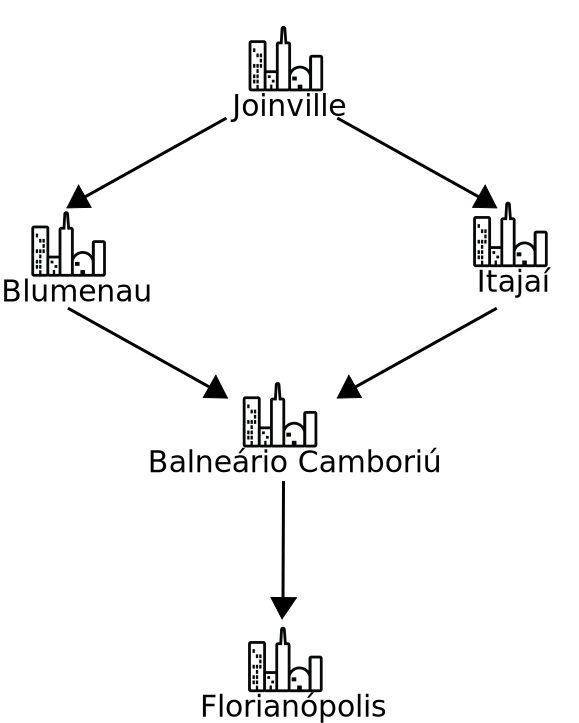
\includegraphics[height=6cm]{cities}
	\end{center}
\end{frame}

\begin{frame}[t]{Inferência em LPO - Passo \#1 = Definir o domínio}	
	$$\begin{array}{lll}
	(1) & estrada(joinville, itajai) & \\
	(2) & estrada(joinville, blumenau) & \\
	(3) & estrada(itajai, balneariocamboriu) & \\
	(4) & estrada(blumenau, balneariocamboriu) & \\
	(5) & estrada(balneariocamboriu, florianopolis) & \\
	\hline
	\end{array}$$	
\end{frame}

\begin{frame}[t]{Inferência em LPO - Passo \#2 = Definir as regras}	
	\begin{tiny}
	$$\begin{array}{lll}
	(1) & estrada(joinville, itajai) & \\
	(2) & estrada(joinville, blumenau) & \\
	(3) & estrada(itajai, balneariocamboriu) & \\
	(4) & estrada(blumenau, balneariocamboriu) & \\
	(5) & estrada(balneariocamboriu, florianopolis) & \\
	(6) & \forall Origem ~\exists Destino: estrada(Origem, Destino) \rightarrow caminho(Origem, Destino) & \\
	(7) & \forall Origem ~\exists Destino: estrada(Origem, Escala) \wedge caminho(Escala, Destino) \rightarrow caminho(Origem, Destino) & \\
	\hline
	\end{array}$$	
	\end{tiny}
\end{frame}

\begin{frame}[t]{Inferência em LPO - Passo \#3 = Definição da Hipótese}	
	\begin{tiny}
	$$\begin{array}{lll}
	(1) & estrada(joinville, itajai) & \\
	(2) & estrada(joinville, blumenau) & \\
	(3) & estrada(itajai, balneariocamboriu) & \\
	(4) & estrada(blumenau, balneariocamboriu) & \\
	(5) & estrada(balneariocamboriu, florianopolis) & \\
	(6) & \forall Origem ~\exists Destino: estrada(Origem, Destino) \rightarrow caminho(Origem, Destino) & \\
	(7) & \forall Origem ~\exists Destino: estrada(Origem, Escala) \wedge caminho(Escala, Destino) \rightarrow caminho(Origem, Destino) & \\
	\hline
	\end{array}$$	
	\end{tiny}

	$$\vdash caminho(joinville, florianopolis)$$
\end{frame}

\begin{frame}[t]{Inferência em LPO - Passo \#4 = Inferência}	
	\begin{tiny}
	$$\begin{array}{lll}
	(1) & estrada(joinville, itajai) & \\
	(2) & estrada(joinville, blumenau) & \\
	(3) & estrada(itajai, balneariocamboriu) & \\
	(4) & estrada(blumenau, balneariocamboriu) & \\
	(5) & estrada(balneariocamboriu, florianopolis) & \\
	(6) & \forall Origem ~\exists Destino: estrada(Origem, Destino) \rightarrow caminho(Origem, Destino) & \\
	(7) & \forall Origem ~\exists Destino: estrada(Origem, Escala) \wedge caminho(Escala, Destino) & \\
	& \rightarrow caminho(Origem, Destino) & \\
	\hline
	(8) & estrada(joinville, itajai) \wedge caminho(itajai, florianopolis) \rightarrow caminho(joinville, florianopolis) & \mathbf{(7)~por~(PU)~\begin{array}{l} Origem/joinville \\ Escala/itajai \\ Destino/florianopolis \end{array}}
	\end{array}$$	
	\end{tiny}

	$$\vdash caminho(joinville, florianopolis)$$
\end{frame}

\begin{frame}[t]{Inferência em LPO - Passo \#4 = Inferência}	
	\begin{tiny}
	$$\begin{array}{lll}
	(1) & estrada(joinville, itajai) & \\
	(2) & estrada(joinville, blumenau) & \\
	(3) & estrada(itajai, balneariocamboriu) & \\
	(4) & estrada(blumenau, balneariocamboriu) & \\
	(5) & estrada(balneariocamboriu, florianopolis) & \\
	(6) & \forall Origem ~\exists Destino: estrada(Origem, Destino) \rightarrow caminho(Origem, Destino) & \\
	(7) & \forall Origem ~\exists Destino: estrada(Origem, Escala) \wedge caminho(Escala, Destino) & \\
	& \rightarrow caminho(Origem, Destino) & \\
	\hline
	(8) & estrada(joinville, itajai) \wedge caminho(itajai, florianopolis) \rightarrow caminho(joinville, florianopolis) & \mathbf{(7)~por~(PU)~\begin{array}{l} Origem/joinville \\ Escala/itajai \\ Destino/florianopolis \end{array}} \\
	(9) & estrada(itajai, balneariocamboriu) \wedge caminho(balneariocamboriu, florianopolis) & \\
	 &  \rightarrow caminho(itajai, florianopolis) &  \mathbf{(7)~por~(PU)~\begin{array}{l} Origem/itajai\\ Escala/balneariocamboriu \\ Destino/florianopolis \end{array}} \\
	\end{array}$$	
	\end{tiny}

	$$\vdash caminho(joinville, florianopolis)$$
\end{frame}

\begin{frame}[t]{Inferência em LPO - Passo \#4 = Inferência}	
	\begin{tiny}
	$$\begin{array}{lll}
	(1) & estrada(joinville, itajai) & \\
	(2) & estrada(joinville, blumenau) & \\
	(3) & estrada(itajai, balneariocamboriu) & \\
	(4) & estrada(blumenau, balneariocamboriu) & \\
	(5) & estrada(balneariocamboriu, florianopolis) & \\
	(6) & \forall Origem ~\exists Destino: estrada(Origem, Destino) \rightarrow caminho(Origem, Destino) & \\
	(7) & \forall Origem ~\exists Destino: estrada(Origem, Escala) \wedge caminho(Escala, Destino) & \\
	& \rightarrow caminho(Origem, Destino) & \\
	\hline
	(8) & estrada(joinville, itajai) \wedge caminho(itajai, florianopolis) \rightarrow caminho(joinville, florianopolis) & \mathbf{(7)~por~(PU)~\begin{array}{l} Origem/joinville \\ Escala/itajai \\ Destino/florianopolis \end{array}} \\
	(9) & estrada(itajai, balneariocamboriu) \wedge caminho(balneariocamboriu, florianopolis) & \\
	 &  \rightarrow caminho(itajai, florianopolis) &  \mathbf{(7)~por~(PU)~\begin{array}{l} Origem/itajai\\ Escala/balneariocamboriu \\ Destino/florianopolis \end{array}} \\
	(10) & estrada(balneariocamboriu, florianopolis) \rightarrow caminho(balneariocamboriu, florianopolis) & \mathbf{(6)~por~(PU)~\begin{array}{l} Origem/balneariocamboriu \\ Destino/florianopolis \end{array}} \\
	\end{array}$$	
	\end{tiny}

	$$\vdash caminho(joinville, florianopolis)$$
\end{frame}

\begin{frame}[t]{Inferência em LPO - Passo \#4 = Inferência}	
	\begin{tiny}
	$$\begin{array}{lll}
	(1) & estrada(joinville, itajai) & \\
	(2) & estrada(joinville, blumenau) & \\
	(3) & estrada(itajai, balneariocamboriu) & \\
	(4) & estrada(blumenau, balneariocamboriu) & \\
	(5) & estrada(balneariocamboriu, florianopolis) & \\
	(6) & \forall Origem ~\exists Destino: estrada(Origem, Destino) \rightarrow caminho(Origem, Destino) & \\
	(7) & \forall Origem ~\exists Destino: estrada(Origem, Escala) \wedge caminho(Escala, Destino) & \\
	& \rightarrow caminho(Origem, Destino) & \\
	\hline
	(8) & estrada(joinville, itajai) \wedge caminho(itajai, florianopolis) \rightarrow caminho(joinville, florianopolis) & \mathbf{(7)~por~(PU)~\begin{array}{l} Origem/joinville \\ Escala/itajai \\ Destino/florianopolis \end{array}} \\
	(9) & estrada(itajai, balneariocamboriu) \wedge caminho(balneariocamboriu, florianopolis) & \\
	 &  \rightarrow caminho(itajai, florianopolis) &  \mathbf{(7)~por~(PU)~\begin{array}{l} Origem/itajai\\ Escala/balneariocamboriu \\ Destino/florianopolis \end{array}} \\
	(10) & estrada(balneariocamboriu, florianopolis) \rightarrow caminho(balneariocamboriu, florianopolis) & \mathbf{(6)~por~(PU)~\begin{array}{l} Origem/balneariocamboriu \\ Destino/florianopolis \end{array}} \\
	(11) & caminho(balneariocamboriu, florianopolis) & \mathbf{(5,10) ~por~(MP)} \\
	\end{array}$$	
	\end{tiny}

	$$\vdash caminho(joinville, florianopolis)$$
\end{frame}

\begin{frame}[t]{Inferência em LPO - Passo \#4 = Inferência}	
	\begin{tiny}
	$$\begin{array}{lll}
	(1) & estrada(joinville, itajai) & \\
	(2) & estrada(joinville, blumenau) & \\
	(3) & estrada(itajai, balneariocamboriu) & \\
	(4) & estrada(blumenau, balneariocamboriu) & \\
	(5) & estrada(balneariocamboriu, florianopolis) & \\
	(6) & \forall Origem ~\exists Destino: estrada(Origem, Destino) \rightarrow caminho(Origem, Destino) & \\
	(7) & \forall Origem ~\exists Destino: estrada(Origem, Escala) \wedge caminho(Escala, Destino) & \\
	& \rightarrow caminho(Origem, Destino) & \\
	\hline
	(8) & estrada(joinville, itajai) \wedge caminho(itajai, florianopolis) \rightarrow caminho(joinville, florianopolis) & \mathbf{(7)~por~(PU)~\begin{array}{l} Origem/joinville \\ Escala/itajai \\ Destino/florianopolis \end{array}} \\
	(9) & estrada(itajai, balneariocamboriu) \wedge caminho(balneariocamboriu, florianopolis) & \\
	 &  \rightarrow caminho(itajai, florianopolis) &  \mathbf{(7)~por~(PU)~\begin{array}{l} Origem/itajai\\ Escala/balneariocamboriu \\ Destino/florianopolis \end{array}} \\
	(10) & estrada(balneariocamboriu, florianopolis) \rightarrow caminho(balneariocamboriu, florianopolis) & \mathbf{(6)~por~(PU)~\begin{array}{l} Origem/balneariocamboriu \\ Destino/florianopolis \end{array}} \\
	(11) & caminho(balneariocamboriu, florianopolis) & \mathbf{(5,10) ~por~(MP)} \\
	(12) & estrada(itajai, balneariocamboriu) \wedge caminho(balneariocamboriu, florianopolis) & \mathbf{(3, 11)~por~(CONJ)} \\
	\end{array}$$	
	\end{tiny}

	$$\vdash caminho(joinville, florianopolis)$$
\end{frame}

\begin{frame}[t]{Inferência em LPO - Passo \#4 = Inferência}	
	\begin{tiny}
	$$\begin{array}{lll}
	(1) & estrada(joinville, itajai) & \\
	(2) & estrada(joinville, blumenau) & \\
	(3) & estrada(itajai, balneariocamboriu) & \\
	(4) & estrada(blumenau, balneariocamboriu) & \\
	(5) & estrada(balneariocamboriu, florianopolis) & \\
	(6) & \forall Origem ~\exists Destino: estrada(Origem, Destino) \rightarrow caminho(Origem, Destino) & \\
	(7) & \forall Origem ~\exists Destino: estrada(Origem, Escala) \wedge caminho(Escala, Destino) & \\
	& \rightarrow caminho(Origem, Destino) & \\
	\hline
	(8) & estrada(joinville, itajai) \wedge caminho(itajai, florianopolis) \rightarrow caminho(joinville, florianopolis) & \mathbf{(7)~por~(PU)~\begin{array}{l} Origem/joinville \\ Escala/itajai \\ Destino/florianopolis \end{array}} \\
	(9) & estrada(itajai, balneariocamboriu) \wedge caminho(balneariocamboriu, florianopolis) & \\
	 &  \rightarrow caminho(itajai, florianopolis) &  \mathbf{(7)~por~(PU)~\begin{array}{l} Origem/itajai\\ Escala/balneariocamboriu \\ Destino/florianopolis \end{array}} \\
	(10) & estrada(balneariocamboriu, florianopolis) \rightarrow caminho(balneariocamboriu, florianopolis) & \mathbf{(6)~por~(PU)~\begin{array}{l} Origem/balneariocamboriu \\ Destino/florianopolis \end{array}} \\
	(11) & caminho(balneariocamboriu, florianopolis) & \mathbf{(5,10) ~por~(MP)} \\
	(12) & estrada(itajai, balneariocamboriu) \wedge caminho(balneariocamboriu, florianopolis) & \mathbf{(3, 11)~por~(CONJ)} \\
	(13) & caminho(itajai, florianopolis) & \mathbf{(9, 12) ~por~(MP)} \\
	\end{array}$$	
	\end{tiny}

	$$\vdash caminho(joinville, florianopolis)$$
\end{frame}

\begin{frame}[t]{Inferência em LPO - Passo \#4 = Inferência}	
	\begin{tiny}
	$$\begin{array}{lll}
	(1) & estrada(joinville, itajai) & \\
	(2) & estrada(joinville, blumenau) & \\
	(3) & estrada(itajai, balneariocamboriu) & \\
	(4) & estrada(blumenau, balneariocamboriu) & \\
	(5) & estrada(balneariocamboriu, florianopolis) & \\
	(6) & \forall Origem ~\exists Destino: estrada(Origem, Destino) \rightarrow caminho(Origem, Destino) & \\
	(7) & \forall Origem ~\exists Destino: estrada(Origem, Escala) \wedge caminho(Escala, Destino) & \\
	& \rightarrow caminho(Origem, Destino) & \\
	\hline
	(8) & estrada(joinville, itajai) \wedge caminho(itajai, florianopolis) \rightarrow caminho(joinville, florianopolis) & \mathbf{(7)~por~(PU)~\begin{array}{l} Origem/joinville \\ Escala/itajai \\ Destino/florianopolis \end{array}} \\
	(9) & estrada(itajai, balneariocamboriu) \wedge caminho(balneariocamboriu, florianopolis) & \\
	 &  \rightarrow caminho(itajai, florianopolis) &  \mathbf{(7)~por~(PU)~\begin{array}{l} Origem/itajai\\ Escala/balneariocamboriu \\ Destino/florianopolis \end{array}} \\
	(10) & estrada(balneariocamboriu, florianopolis) \rightarrow caminho(balneariocamboriu, florianopolis) & \mathbf{(6)~por~(PU)~\begin{array}{l} Origem/balneariocamboriu \\ Destino/florianopolis \end{array}} \\
	(11) & caminho(balneariocamboriu, florianopolis) & \mathbf{(5,10) ~por~(MP)} \\
	(12) & estrada(itajai, balneariocamboriu) \wedge caminho(balneariocamboriu, florianopolis) & \mathbf{(3, 11)~por~(CONJ)} \\
	(13) & caminho(itajai, florianopolis) & \mathbf{(9, 12) ~por~(MP)} \\
	(14) & estrada(joinville, itajai) \wedge caminho(itajai, florianopolis) & \mathbf{(1, 13) ~por~(CONJ)} \\
	\end{array}$$	
	\end{tiny}

	$$\vdash caminho(joinville, florianopolis)$$
\end{frame}

\begin{frame}[t]{Inferência em LPO - Passo \#4 = Inferência}	
	\begin{tiny}
	$$\begin{array}{lll}
	(1) & estrada(joinville, itajai) & \\
	(2) & estrada(joinville, blumenau) & \\
	(3) & estrada(itajai, balneariocamboriu) & \\
	(4) & estrada(blumenau, balneariocamboriu) & \\
	(5) & estrada(balneariocamboriu, florianopolis) & \\
	(6) & \forall Origem ~\exists Destino: estrada(Origem, Destino) \rightarrow caminho(Origem, Destino) & \\
	(7) & \forall Origem ~\exists Destino: estrada(Origem, Escala) \wedge caminho(Escala, Destino) & \\
	& \rightarrow caminho(Origem, Destino) & \\
	\hline
	(8) & estrada(joinville, itajai) \wedge caminho(itajai, florianopolis) \rightarrow caminho(joinville, florianopolis) & \mathbf{(7)~por~(PU)~\begin{array}{l} Origem/joinville \\ Escala/itajai \\ Destino/florianopolis \end{array}} \\
	(9) & estrada(itajai, balneariocamboriu) \wedge caminho(balneariocamboriu, florianopolis) & \\
	 &  \rightarrow caminho(itajai, florianopolis) &  \mathbf{(7)~por~(PU)~\begin{array}{l} Origem/itajai\\ Escala/balneariocamboriu \\ Destino/florianopolis \end{array}} \\
	(10) & estrada(balneariocamboriu, florianopolis) \rightarrow caminho(balneariocamboriu, florianopolis) & \mathbf{(6)~por~(PU)~\begin{array}{l} Origem/balneariocamboriu \\ Destino/florianopolis \end{array}} \\
	(11) & caminho(balneariocamboriu, florianopolis) & \mathbf{(5,10) ~por~(MP)} \\
	(12) & estrada(itajai, balneariocamboriu) \wedge caminho(balneariocamboriu, florianopolis) & \mathbf{(3, 11)~por~(CONJ)} \\
	(13) & caminho(itajai, florianopolis) & \mathbf{(9, 12) ~por~(MP)} \\
	(14) & estrada(joinville, itajai) \wedge caminho(itajai, florianopolis) & \mathbf{(1, 13) ~por~(CONJ)} \\
	(15) & caminho(joinville, florianopolis) & \mathbf{(8, 14)~por~(MP)}
	\end{array}$$	
	\end{tiny}

	$$\vdash caminho(joinville, florianopolis)$$
\end{frame}


\begin{frame}[t]{Inferência em LPO - Exercício}	
	Traduzir os conhecimentos abaixo para LPO (fatos ou regras):

	\begin{enumerate}
	\item Marcos era um homem
	\item Todos os homens e mulheres são pessoas
	\item Marcos nasceu em Pompeia
	\item Todos os que nasceram em Pompeia eram romanos
	\item Cesar era um soberano
	\item Todos os romanos eram leais a Cesar ou o odiavam
	\item As pessoas só tentam assassinar soberanos aos quais não são leais
	\item Marcos tentou assassinar Cesar
	\end{enumerate}

	\vskip 0.5cm

	{\bf Prove que:} Marcos odeia Cesar 
\end{frame}


\begin{frame}[t]{Inferência em LPO - Exercício}
	\begin{tiny}	
	$$\begin{array}{lll}
	(1) & homem(marcos) & \\
	(2) & \forall X: ~homem(X) \vee mulher(X) \rightarrow pessoa(X) & \\
	(3) & pompeano(marcos) & \\
	(4) & \forall X: ~pompeano(X) \rightarrow romano(X) & \\
	(5) & soberano(cesar) & \\
	(6) & \forall X:~romano(X) \rightarrow leal\_a(X, cesar) \vee odeia(X, cesar) & \\
	(7) & \forall X~\exists Y:~ pessoa(X) \wedge soberano(Y) \wedge tenta\_assassinar(X,Y) \rightarrow \sim leal\_a(X,Y) & \\
	(8) & tenta\_assassinar(marcos, cesar) & \\
	\hline
	\end{array}$$	
	\end{tiny}

	$$\vdash odeia(marcos, cesar)$$
\end{frame}


\begin{frame}[t]{Inferência em LPO - Exercício}
	\begin{tiny}	
	$$\begin{array}{lll}
	(1) & homem(marcos) & \\
	(2) & \forall X: ~homem(X) \vee mulher(X) \rightarrow pessoa(X) & \\
	(3) & pompeano(marcos) & \\
	(4) & \forall X: ~pompeano(X) \rightarrow romano(X) & \\
	(5) & soberano(cesar) & \\
	(6) & \forall X:~romano(X) \rightarrow leal\_a(X, cesar) \vee odeia(X, cesar) & \\
	(7) & \forall X~\exists Y:~ pessoa(X) \wedge soberano(Y) \wedge tenta\_assassinar(X,Y) \rightarrow \sim leal\_a(X,Y) & \\
	(8) & tenta\_assassinar(marcos, cesar) & \\
	\hline
	(9) & pessoa(marcos) \wedge soberano(cesar) \wedge tenta\_assassinar(marcos, cesar) & \\
	     & \rightarrow\sim leal\_a(marcos, cesar) & \mathbf{(7) ~por~(PU)~\begin{array}{l} X/marcos \\ Y/cesar \end{array}} \\
	(10) & homem(marcos) \vee mulher(marcos) \rightarrow pessoa(marcos) & \mathbf{(2) ~por~(PU) ~~  X/marcos } \\
	(11) & homem(marcos) \vee mulher(marcos)  & \mathbf{(1) ~por~(AD)} \\
	(12) & pessoa(marcos) & \mathbf{(10, 11) ~por~(MP)} \\
	(13) & pessoa(marcos) \wedge soberano(cesar) & \mathbf{(5, 12) ~por~(CONJ)} \\
	(14) & pessoa(marcos) \wedge soberano(cesar) \wedge tenta\_assassinar(marcos, cesar) & \mathbf{(8,13) ~por~(CONJ)} \\
	(15) &\sim leal\_a(marcos, cesar) & \mathbf{(9,14) ~por~(MP)} \\
	(16) & pompeano(marcos) \rightarrow romano(marcos) & \mathbf{(4) ~por~(PU) ~~X/marcos} \\
	(17) & romano(marcos) & \mathbf{(3, 16) ~por~(MP)} \\
	(18) & romano(marcos) \rightarrow leal\_a(marcos, cesar) \vee odeia(marcos, cesar) & \mathbf{(6) ~por~(PU)~~X/marcos} \\
	(19) & leal\_a(marcos, cesar) \vee odeia(marcos, cesar) & \mathbf{(17, 18) ~por~(MP)} \\
	(20) & odeia(marcos, cesar) & \mathbf{(15, 19) ~por~(SD)} 
	\end{array}$$	
	\end{tiny}

	$$\vdash odeia(marcos, cesar)$$
\end{frame}



\begin{frame}[t]{Resumindo os Elementos da Lógica de Predicados}
	\begin{itemize} 
	\itemsep 0.3cm
	\item Há fatos sobre objetos atômicos: $\{a, b, ..., 0, 1, ...,V, F, ...\}$
	\item Os objetos são pertencentes a um dado domínio: ($D$)
%	\item Estes objetos podem constituir uma classe predicativa
	\item Assim,  há {\bf predicados} que  estabelecem relações entre os objetos
	
	\item Estas relações ou predicados operam sobre objetos de domínios: $$D = D_1 \cup D_2 \cup\ldots\cup D_N$$
	\item Há o conceito de interpretação ou validade da fórmula predicativa, dada por: $\Phi (predicado) = \{V, F\}$
  \item Há ainda, os functores ou funções lógicas, os quais são mapeados em $D$

\item Em resumo, adicione o conceito de conjuntos à lógica proposicional, e define-se
uma lógica mais poderosa: a {\bf lógica de primeira-ordem}.

	\end{itemize}
\end{frame}


\begin{frame}[t]{Exercício}

Considere o seguinte conjunto de f\'ormulas: 
%%%{\bf \textcolor{red}{é boa esta questão ... manteria !}}

\vspace{13pt}

\begin{tabular}{ll}
 \hline \hline
1. &  $\forall x\forall y (q(x,y) \wedge r(y) \rightarrow p(y)) $ \\
2. &  $\forall x  (q(x,x) \rightarrow p(x))  $ \\
3. &  $\forall x \exists y ( s(x) \rightarrow q(x,y)) $ \\
4. &  $r(b)$ \\ 
5. &  $s(a)$ \\
6. &  $s(b)$  \\ 
\hline \hline
\end{tabular}

\vspace{13pt}

Utilizando as propriedades da LPO (por exemplo: PU, GU, GE e PE), demonstre: $\sim p(a)$ \textbf{ ou } $p(a)$ e $\sim p(b)$ \textbf{ ou } $p(b)$. O domínio é dado por $D=\{a,b\}$. 


\end{frame}
